\chapter{Data Collection}
For the extended project, eight participants tested the prototype (five males, three females; average age 23). It should be noted that it was considered as an early test, since it was still in a very early stage of development.

Figures \ref{fig:1}, \ref{fig:2}, \ref{fig:3}, \ref{fig:4}, \ref{fig:5}, \ref{fig:6}, \ref{fig:7}, \ref{fig:8}, \ref{fig:9} show the results from the tests. Since the tests also included other elements in the questionnaire (such as collecting data on demographics, emotions, as well as specific questions about the gameplay), not all of the questions mentioned in Section \ref{qustionnaire} have been included. Otherwise, the questionnaire would be too long, with the risk of participants growing tired and not taking the questions seriously.

The scale was shown as follows:

\begin{itemize}
\item 1 = Strongly disagree
\item 2 = Disagree
\item 3 = Neither agree nor disagree
\item 4 = Agree
\item 5 = Strongly agree
\end{itemize}

\begin{figure}[htbp]
\centering
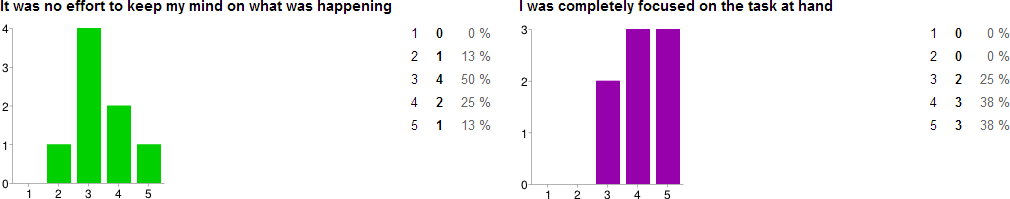
\includegraphics[width=1.0\textwidth]{Pictures/flow_1_focus}
\caption{Flow results.}
\label{fig:1}
\end{figure}

\begin{figure}[htbp]
\centering
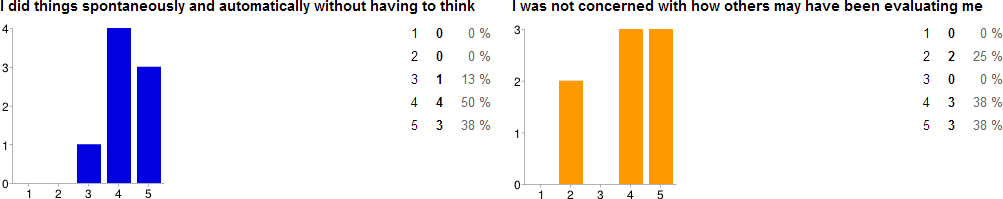
\includegraphics[width=1.0\textwidth]{Pictures/flow_2_social}
\caption{Flow results.}
\label{fig:2}
\end{figure}

\begin{figure}[htbp]
\centering
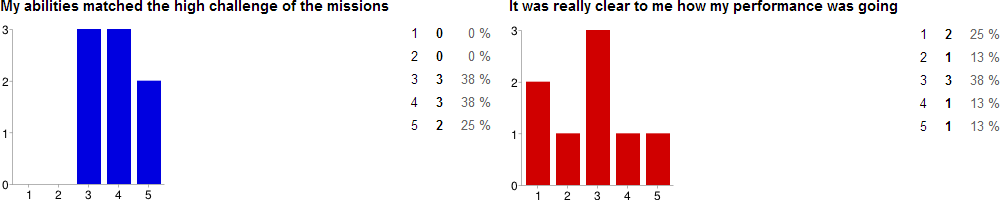
\includegraphics[width=1.0\textwidth]{Pictures/flow_3_senseOfControl}
\caption{Flow results.}
\label{fig:3}
\end{figure}

\begin{figure}[htbp]
\centering
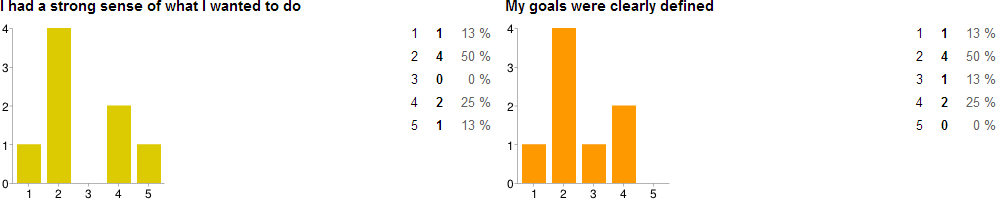
\includegraphics[width=1.0\textwidth]{Pictures/flow_4_senseOfControl}
\caption{Flow results.}
\label{fig:4}
\end{figure}

\begin{figure}[htbp]
\centering
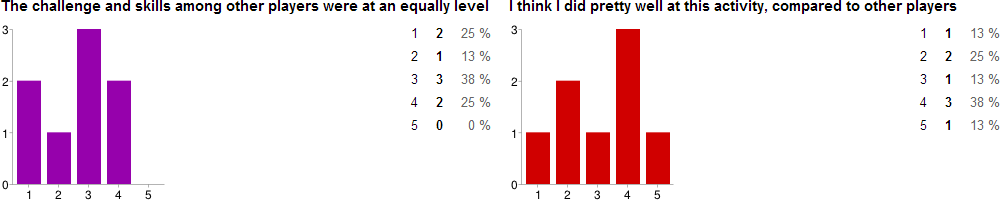
\includegraphics[width=1.0\textwidth]{Pictures/flow_5_senseOfControl}
\caption{Flow and IMI results.}
\label{fig:5}
\end{figure}

\begin{figure}[htbp]
\centering
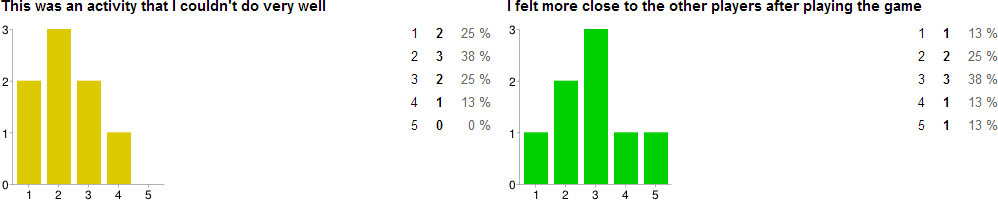
\includegraphics[width=1.0\textwidth]{Pictures/imi_1}
\caption{IMI results.}
\label{fig:6}
\end{figure}

\begin{figure}[htbp]
\centering
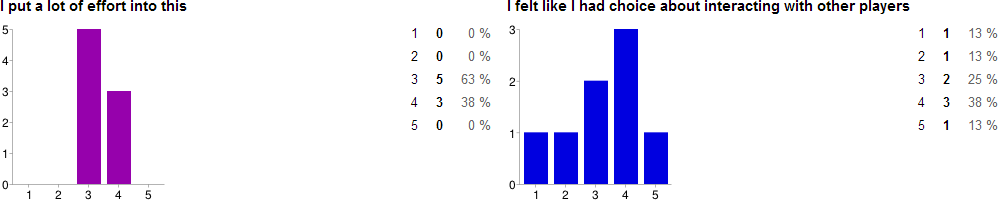
\includegraphics[width=1.0\textwidth]{Pictures/imi_2}
\caption{IMI results.}
\label{fig:7}
\end{figure}

\begin{figure}[htbp]
\centering
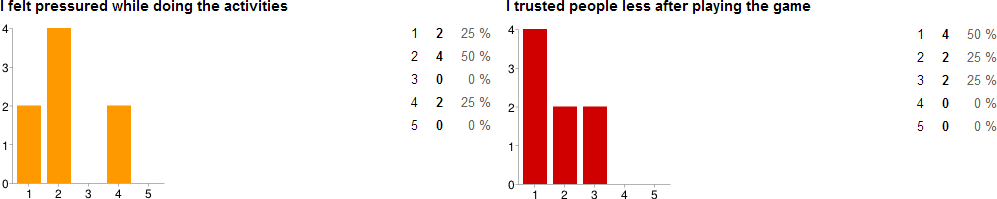
\includegraphics[width=1.0\textwidth]{Pictures/imi_3}
\caption{IMI results.}
\label{fig:8}
\end{figure}

\begin{figure}[htbp]
\centering
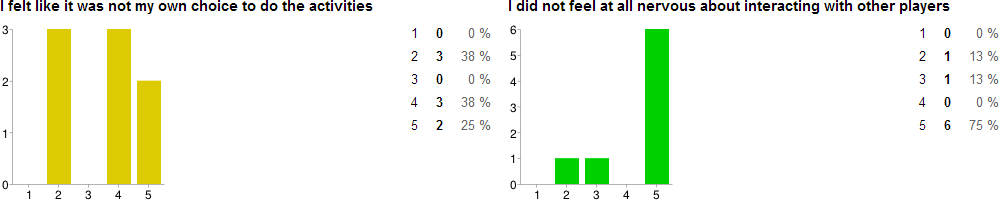
\includegraphics[width=1.0\textwidth]{Pictures/imi_4}
\caption{IMI results.}
\label{fig:9}
\end{figure}